% Provenance (never printed): old premiere S material on the history of plate
% tectonics (from continental drift to seafloor spreading: the ridges, the
% magnetic stripes, the ages of the drilled floor); see
% sources/book2/PROVENANCE.md. Profiles are computed in
% figdata/grade-11/magnetic_stripes.py, the age map in seafloor_age.py, the
% drilling fit in sediment_ages.py.
\chapter{Da deriva continental à expansão do assoalho oceânico}\label{ch:g11:drift-to-spreading}

No início dos anos 1950, no laboratório Lamont da Universidade Columbia, uma
jovem geóloga chamada Marie Tharp estava sentada diante de longas fileiras
de números. Cada um era uma profundidade do Atlântico Norte, medida pelo
ecobatímetro de um navio, uma depois da outra ao longo da rota do navio.
Colocando-as num gráfico uma a uma, ela desenhou a forma do fundo do oceano
ao longo das rotas dos navios que haviam atravessado o oceano. No meio do
oceano, o fundo se erguia numa cadeia de montanhas --- e, em cada rota, ao
longo da crista da cadeia, o fundo descia de novo numa fenda profunda, como
se as montanhas tivessem sido partidas ao meio. Este capítulo acompanha como
essas medições do fundo do oceano transformaram uma ideia rejeitada, a
deriva dos continentes, numa teoria: o assoalho oceânico é fabricado nas
dorsais e se afasta delas, e ele leva nas suas rochas um registro da sua
própria idade.
% ledger: aip:tharp, aip:featureless, usgs:echo-sounding

\begin{recall}
A deriva continental é a ideia de que os continentes se movem; Alfred
Wegener a defendeu a partir de 1912 com o encaixe das costas, os fósseis, as
rochas e os climas antigos, mas não soube dizer o que os movia. A superfície
da Terra é feita de placas rígidas, que se encontram em limites divergentes,
convergentes e transformantes; elas se movem alguns centímetros por ano, e
$\qty{1}{cm}$ por ano são $\qty{10}{km}$ por milhão de anos (Livro 1, 7º
ano). O fundo do oceano tem a sua plataforma continental, as suas planícies
abissais, as suas dorsais e as suas fossas (Livro 1, 8º ano). A Terra tem um
campo magnético, com um polo norte e um polo sul magnéticos, que a agulha de
uma bússola segue; um pulso de som enviado na água volta como um eco depois
de um tempo que dá a distância (os livros de física).
\end{recall}

\section{Por que a deriva foi rejeitada}

As provas de Wegener mostravam que os continentes já tinham estado unidos. O
que elas não mostravam era como eles poderiam ter se movido. Wegener
imaginava os continentes abrindo caminho pela rocha do fundo do oceano, e os
físicos responderam que nenhuma força conhecida podia empurrar um continente
através de rocha sólida sem esmagá-lo. Durante meio século, a maioria dos
geólogos concluiu que os continentes não tinham se movido de modo algum.
% ledger: usgs:wegener-1912, usgs:jeffreys (Book 1 rows)

Faltavam duas coisas. A primeira era um mecanismo. A segunda, que levou à
primeira, era o conhecimento do fundo dos oceanos, que cobre a maior parte
da superfície da Terra e que, em 1912, quase ninguém tinha visto: supunha-se
que fosse uma planície quase sem relevo.
% ledger: aip:tharp, aip:featureless

\section{Mapear o fundo do oceano}

Um ecobatímetro envia um pulso curto de som do casco de um navio até o fundo
do mar e cronometra o seu eco. O som se propaga na água do mar a cerca de
\qty{1500}{m/s}; o pulso desce e volta, de modo que um atraso $t$ significa
uma profundidade
\[
  d = \frac{v\,t}{2}.
\]
Um atraso de \qty{6.0}{s}, por exemplo, significa $1500 \times 6.0/2 =
\qty{4500}{m}$ de água. No século XIX, as profundidades eram medidas uma de
cada vez, descendo uma linha com peso até o fundo. Depois da Primeira Guerra
Mundial, os ecobatímetros tomaram o seu lugar, e os registros dos seus ecos
mostraram um fundo muito mais acidentado do que se pensava; nos anos 1950,
levantamentos feitos por navios de muitos países mostraram que uma grande
cadeia de montanhas no fundo do oceano dá quase a volta inteira à Terra.
% ledger: noaa:sound-seawater, usgs:echo-sounding, usgs:line-soundings

\begin{history}[Marie Tharp e o vale de rifte, 1952]
% ledger: aip:tharp, aip:featureless
A partir de 1947, o geofísico Bruce Heezen havia reunido perfis de
ecobatimetria através do Atlântico Norte. Marie Tharp, que na época não
tinha permissão para embarcar nos navios de pesquisa, transformou o que ela
mais tarde chamou de ``intermináveis fileiras de números de sondagem'' em
desenhos do fundo do mar. Em 1952, com as rotas leste--oeste dispostas em
ordem de norte a sul, ela viu que uma feição se alinhava de rota em rota:
uma fenda ao longo da crista da Dorsal Mesoatlântica, um vale de rifte.
Heezen a princípio achou que era um erro. Depois, os epicentros dos
terremotos do Atlântico, colocados no mapa na mesma escala, mostraram-se
situados no próprio vale de rifte. O mapa do fundo dos oceanos do mundo de
Tharp e Heezen, pintado pelo artista Heinrich Berann em 1977, deu às pessoas
a primeira imagem realista do fundo do oceano; em 1997, a Biblioteca do
Congresso dos Estados Unidos a incluiu entre os quatro grandes cartógrafos
do século XX.
\end{history}

As dorsais oceânicas formam um sistema único, quase contínuo, de cerca de
\qty{65000}{km} de comprimento, mais de nove décimos dele debaixo da água; a
crista fica em média a \qty{2500}{m} abaixo da superfície. Ao longo da lenta
Dorsal Mesoatlântica, a crista é cortada por um vale de rifte; ao longo da
Dorsal do Pacífico Oriental, mais rápida, ela é um cume liso e suave. Os
terremotos dos oceanos seguem as dorsais de perto. Tudo apontava a dorsal
como um lugar onde alguma coisa estava acontecendo --- mas o quê?
% ledger: noaa:ridge, aip:tharp

\section{A expansão do assoalho oceânico}

\begin{history}[Hess e a esteira rolante, 1962]
% ledger: usgs:hess, hess:1962
Em 1962, Harry Hess, geólogo da Universidade de Princeton e almirante da
reserva naval, publicou \emph{History of Ocean Basins}. Ele propôs que a
rocha quente sobe sob as dorsais e se torna novo assoalho oceânico, que
então se afasta dos dois lados como uma esteira rolante e volta a afundar no
manto nas fossas. Robert Dietz, que chegou à mesma ideia, deu-lhe o nome:
\omterm{def:g11:drift-to-spreading:spreading}{expansão do assoalho oceânico}. A ideia explicava por que a Terra não cresce,
embora novo assoalho esteja sempre sendo fabricado, por que há tão pouco
sedimento no fundo do oceano, e por que as rochas do fundo do oceano são
muito mais jovens que as dos continentes.
\end{history}

\begin{definition}[Expansão do assoalho oceânico]\label{def:g11:drift-to-spreading:spreading}
A \emph{expansão do assoalho oceânico}\index{expansao do assoalho oceanico@expansão do assoalho oceânico} é o processo pelo qual
um novo assoalho oceânico se forma ao longo da crista de uma dorsal
oceânica, onde a rocha fundida sobe do manto e se solidifica, e depois se
afasta da dorsal dos dois lados, de modo que o assoalho oceânico fica mais
velho com a distância à dorsal.
\end{definition}

\begin{definition}[Taxa de expansão]\label{def:g11:drift-to-spreading:spreading-rate}
A \emph{taxa de expansão total}\index{taxa de expansao@taxa de expansão} de
uma dorsal é a velocidade com que as duas placas de cada lado dela se
afastam uma da outra. A \emph{semitaxa de expansão} é a velocidade com que o
assoalho de um lado se afasta do eixo da dorsal. Quando a expansão é
simétrica, a taxa total é o dobro da semitaxa.
\end{definition}

As dorsais se expandem a velocidades muito diferentes. A Dorsal
Mesoatlântica se abre a \qtyrange{2}{5}{cm} por ano, a Dorsal do Pacífico
Oriental a \qtyrange{6}{16}{cm} por ano. Do assoalho oceânico que existe
hoje, cerca de um terço foi fabricado em dorsais lentas (taxas totais de
\qtyrange{20}{55}{mm} por ano) e cerca de dois quintos em dorsais rápidas
(\qtyrange{75}{180}{mm} por ano).
% ledger: noaa:ridge, seton:rate-classes

A ideia de Hess era ousada e, no início, tinha poucas provas diretas. As
provas vieram de duas direções inesperadas: o magnetismo do fundo do oceano
e os seus sedimentos.

\section{As inversões magnéticas e o fundo do mar listrado}

\subsection{Uma rocha se lembra do campo}

O basalto do fundo do oceano contém pequenos grãos de magnetita, um óxido de
ferro fortemente magnético. Quando a lava basáltica entra em erupção, ela
está quente demais para guardar qualquer magnetização duradoura; à medida
que esfria, os grãos se magnetizam paralelamente ao campo da Terra à sua
volta, e essa direção fica então travada na rocha.
% ledger: usgs:magnetometers

\begin{definition}[Magnetização remanente; temperatura de Curie]\label{def:g11:drift-to-spreading:remanence}
A \emph{temperatura de Curie}\index{temperatura de Curie} de um mineral
magnético é a temperatura acima da qual ele não consegue manter uma
magnetização própria: cerca de \qty{580}{\celsius} para a magnetita. Uma
rocha cujos grãos magnéticos esfriam abaixo da sua temperatura de Curie no
campo da Terra conserva uma magnetização paralela ao campo daquela época, a
\emph{magnetização remanente}\index{magnetizacao remanente@magnetização remanente}. Ela dura muito depois que o campo mudou,
a menos que a rocha seja aquecida de novo acima da temperatura de Curie.
\end{definition}
% ledger: tarduno:curie

\begin{omfigure}
\begin{tikzpicture}[font=\footnotesize, >={Stealth[length=5pt]}]
  % ground and lava flow
  \fill[lith basalt] (0,0) rectangle (11,0.6);
  \fill[omLithBasalt!45!red!35] (0,0.6) -- (11,0.6) -- (11,1.9) .. controls (9,2.0) and (4,2.15) .. (0,2.05) -- cycle;
  \fill[omLithBasalt!70] (0,1.35) -- (11,1.25) -- (11,1.9) .. controls (9,2.0) and (4,2.15) .. (0,2.05) -- cycle;
  \draw[black!60] (0,1.35) -- (11,1.25);
  \draw[line width=0.8pt] (0,2.05) .. controls (4,2.15) and (9,2.0) .. (11,1.9);
  \draw[black!60] (0,0.6) -- (11,0.6);
  % field lines (northern hemisphere: pointing down to the north)
  \foreach \x in {0.6,2.4,4.2,6.0,7.8,9.6} {
    \draw[->, omDef, line width=0.9pt] (\x,4.0) -- (\x+1.1,2.55);
  }
  \node[anchor=south west, text=omDef] at (0.2,4.05) {o campo magnético da Terra};
  % locked grains in the cooled top
  \foreach \x in {0.5,1.3,...,10.5} {
    \draw[->, black, line width=0.6pt] (\x,1.86) -- (\x+0.25,1.53);
  }
  % random grains in the hot interior
  \foreach \x/\a in {0.6/20,1.5/140,2.3/250,3.2/80,4.0/310,4.9/190,5.7/40,6.6/120,7.4/280,8.3/20,9.1/200,10.0/330} {
    \draw[->, black!55, line width=0.5pt] (\x,0.95) -- ++(\a:0.22);
  }
  \node[anchor=west, align=left] at (11.15,1.75) {resfriada abaixo de \qty{580}{\celsius}: os\\grãos guardam a direção do campo};
  \node[anchor=west, align=left] at (11.15,0.92) {ainda acima de \qty{580}{\celsius}:\\nenhuma magnetização duradoura};
  \node[anchor=west, align=left] at (11.15,0.25) {rocha mais antiga};
  \node[anchor=west] at (9.0,4.25) {norte $\rightarrow$};
\end{tikzpicture}

{\small Um derrame de lava esfriando (esquema, Hemisfério Norte, onde o campo
aponta para o norte e para baixo). O topo do derrame esfriou abaixo da
\omterm{def:g11:drift-to-spreading:remanence}{temperatura de Curie} da magnetita: os seus grãos magnéticos (setas pretas)
conservam a direção do campo. O interior, ainda mais quente, ainda não
registra nada; ele registrará o campo do momento em que esfriar.}
\end{omfigure}

\subsection{O campo se inverte}

No início do século XX, Bernard Brunhes (em 1906) e depois Motonori Matuyama
(nos anos 1920) descobriram que as rochas vulcânicas se dividem em dois
grupos. Em umas, a magnetização aponta no sentido do campo atual; nas
outras, ela aponta no sentido oposto, como se os polos magnéticos norte e
sul tivessem trocado de lugar. O próprio campo tinha se invertido, muitas e
muitas vezes.
% ledger: usgs:reversals

\begin{definition}[Inversão magnética; polaridade normal e inversa]\label{def:g11:drift-to-spreading:reversal}
Uma \emph{inversão magnética}\index{inversao magnetica@inversão magnética} é
uma troca entre os polos magnéticos norte e sul da Terra. Um tempo em que o
campo apontava como hoje é um tempo de \emph{polaridade
normal}\index{polaridade normal}; um tempo em que ele apontava no sentido
oposto, um tempo de \emph{polaridade inversa}\index{polaridade inversa}. Uma
rocha magnetizada durante um desses tempos tem a mesma polaridade.
\end{definition}

Lavas datadas dão a sucessão dos intervalos normais e inversos: a
\emph{escala de tempo de polaridade geomagnética}. Os seus longos intervalos
têm o nome de cientistas que estudaram o magnetismo da Terra (Brunhes,
Matuyama, Gauss, Gilbert); os eventos curtos dentro deles, o dos lugares
onde foram encontrados pela primeira vez.

\begin{omfigure}
\begin{tikzpicture}
\begin{axis}[width=0.92\linewidth, height=3.2cm, xmin=0, xmax=5.5, ymin=-0.9, ymax=1.9,
  axis y line=none, axis x line*=bottom, xtick={0,0.5,...,5.5}, tick label style={font=\small},
  xlabel={idade (milhões de anos)}, label style={font=\small}, clip=false]
\addplot[fill=black, draw=none] table {figdata/out/grade-11-magnetic_stripes-timescale.dat};
\draw[black] (axis cs:0,0) rectangle (axis cs:5.5,1);
\begin{scope}[every node/.style={font=\scriptsize, anchor=south}]
  \node at (axis cs:0.39,1.05) {Brunhes};
  \node at (axis cs:1.68,1.05) {Matuyama};
  \node at (axis cs:3.08,1.05) {Gauss};
  \node at (axis cs:4.74,1.05) {Gilbert};
\end{scope}
\draw[black!60] (axis cs:0.78,1) -- (axis cs:0.78,1.45);
\draw[black!60] (axis cs:2.581,1) -- (axis cs:2.581,1.45);
\draw[black!60] (axis cs:3.58,1) -- (axis cs:3.58,1.45);
\begin{scope}[every node/.style={font=\scriptsize, anchor=north}]
  \node at (axis cs:1.03,-0.05) {Jaramillo};
  \node at (axis cs:1.86,-0.05) {Olduvai};
\end{scope}
\node[font=\scriptsize, anchor=west] at (axis cs:5.55,0.75) {normal};
\node[font=\scriptsize, anchor=west] at (axis cs:5.55,0.25) {(preto)};
\end{axis}
\end{tikzpicture}

{\small A escala de tempo de polaridade geomagnética dos últimos 5.5 milhões
de anos: preto para a \omterm{def:g11:drift-to-spreading:reversal}{polaridade normal}, branco para a inversa. O intervalo
normal atual começou há \num{780000} anos; houve vinte inversões nos últimos
cinco milhões de anos. Dados: Cande e Kent (1995).}
\end{omfigure}
% ledger: ck95:chrons

\subsection{As listras do fundo do oceano}

A partir dos anos 1950, navios rebocaram magnetômetros através dos oceanos e
descobriram que o campo na superfície do mar não era o campo suave esperado
do núcleo da Terra: ele era um pouco mais forte aqui, um pouco mais fraco
ali.
% ledger: usgs:magnetometers

\begin{definition}[Anomalia magnética]\label{def:g11:drift-to-spreading:anomaly}
Num ponto da superfície do mar, a
\emph{anomalia magnética}\index{anomalia magnetica@anomalia magnética} é a intensidade medida do campo magnético menos a
intensidade esperada ali só pelo campo da Terra. Ela é positiva onde as
rochas abaixo se somam ao campo, e negativa onde se opõem a ele. Ela é
pequena em comparação com o próprio campo, e medida em nanoteslas
(\unit{nT}).
\end{definition}

Mapeadas sobre uma região extensa, as anomalias desenharam listras
paralelas à crista da dorsal, alternadamente positivas e negativas, como a
pelagem de uma zebra --- e o padrão de um lado da dorsal era a imagem
espelhada do padrão do outro lado.
% ledger: usgs:magnetometers

\begin{history}[Vine e Matthews, 1963]
% ledger: vm:1963, usgs:magnetometers
Em setembro de 1963, Fred Vine e Drummond Matthews publicaram um artigo
curto na revista \emph{Nature}, \emph{Magnetic anomalies over oceanic
ridges}. Eles juntaram a expansão de Hess e as inversões do campo. Se um
novo assoalho se forma na crista e se afasta enquanto o campo se inverte,
cada faixa de assoalho registra a polaridade da época em que esfriou. O
assoalho se torna uma fita listrada, que se desenrola dos dois lados da
dorsal: anomalias positivas acima das faixas normais, negativas acima das
inversas, a mesma sequência dos dois lados.
\end{history}

\begin{omfigure}
\begin{tikzpicture}
\begin{axis}[hide axis, axis equal image, width=0.94\linewidth, xmin=-320, xmax=420, ymin=-120, ymax=160, clip=false]
  % block faces
  \fill[white] (axis cs:-300,0) -- (axis cs:300,0) -- (axis cs:390,70) -- (axis cs:-210,70) -- cycle;
  \fill[omLithBasalt!25] (axis cs:-300,0) rectangle (axis cs:300,-60);
  \fill[omLithBasalt!45] (axis cs:300,0) -- (axis cs:390,70) -- (axis cs:390,10) -- (axis cs:300,-60) -- cycle;
  \addplot[fill=black!80, draw=none] table {figdata/out/grade-11-magnetic_stripes-block.dat};
  \draw[black] (axis cs:-300,0) -- (axis cs:300,0) -- (axis cs:390,70) -- (axis cs:-210,70) -- cycle;
  \draw[black] (axis cs:-300,0) -- (axis cs:-300,-60) -- (axis cs:300,-60) -- (axis cs:300,0);
  \draw[black] (axis cs:300,-60) -- (axis cs:390,10) -- (axis cs:390,70);
  % ridge axis
  \draw[omRidge, line width=1.6pt] (axis cs:0,0) -- (axis cs:90,70);
  \node[font=\footnotesize, text=omRidge, anchor=south] at (axis cs:90,72) {eixo da dorsal};
  % rising magma
  \fill[red!60!orange, opacity=0.75] (axis cs:-12,-60) -- (axis cs:12,-60) -- (axis cs:3,0) -- (axis cs:-3,0) -- cycle;
  \draw[->, >={Stealth[length=5pt]}, red!70!black, line width=1pt] (axis cs:0,-95) -- (axis cs:0,-62);
  \node[font=\footnotesize, anchor=north] at (axis cs:0,-96) {a rocha fundida sobe};
  % spreading arrows
  \draw[->, >={Stealth[length=6pt]}, line width=1.2pt] (axis cs:-90,100) -- (axis cs:-220,100);
  \draw[->, >={Stealth[length=6pt]}, line width=1.2pt] (axis cs:150,100) -- (axis cs:280,100);
  \node[font=\footnotesize, anchor=south] at (axis cs:-155,103) {mais antigo};
  \node[font=\footnotesize, anchor=south] at (axis cs:215,103) {mais antigo};
  % legend
  \fill[black!80] (axis cs:-300,-100) rectangle (axis cs:-280,-88);
  \node[font=\footnotesize, anchor=west] at (axis cs:-276,-94) {polaridade normal};
  \draw[black] (axis cs:-300,-118) rectangle (axis cs:-280,-106);
  \node[font=\footnotesize, anchor=west] at (axis cs:-276,-112) {polaridade inversa};
\end{axis}
\end{tikzpicture}

{\small O assoalho oceânico listrado (esquema, calculado para uma dorsal que
se expande a \qty{7.5}{cm} por ano de cada lado, ao longo dos últimos 4
milhões de anos). Cada faixa de assoalho conservou a polaridade do campo no
momento em que esfriou no eixo; o padrão de um lado é a imagem espelhada do
outro.}
\end{omfigure}

\begin{proposition}[Distância de uma listra ao eixo]\label{prop:g11:drift-to-spreading:stripe}
Se uma dorsal se expande simetricamente com uma semitaxa constante $u$, o
assoalho que se formou no eixo há um tempo $t$ fica agora a uma distância
\[
  x = u\,t
\]
de cada lado do eixo. Em particular, a fronteira entre duas listras que
registra uma inversão de idade $t$ fica à distância $u\,t$ dos dois lados.
\end{proposition}

\begin{proof}
Um pedaço de assoalho formado no eixo há um tempo $t$ se afastou desde então
do eixo à velocidade $u$, durante o tempo $t$: ele percorreu a distância
$u\,t$. Um pedaço formado no mesmo momento do outro lado do eixo se move no
sentido oposto com a mesma velocidade, e fica à mesma distância. O assoalho
de cada lado de uma fronteira de inversão se formou logo antes e logo depois
da inversão, de modo que a fronteira fica onde está o assoalho de idade $t$:
a $u\,t$.
\end{proof}

As anomalias podem ser calculadas a partir da escala de tempo. Nos perfis
abaixo, a camada magnetizada é uma lâmina de rocha de \qty{1}{km} de
espessura cujo topo fica a \qty{3}{km} abaixo da superfície do mar, dividida
em blocos de \omterm{def:g11:drift-to-spreading:reversal}{polaridade normal} e inversa segundo a proposição; somam-se os
campos de cada bloco na superfície do mar. Acima de uma faixa larga, a
anomalia é mais forte perto das suas bordas, onde a polaridade muda, e mais
fraca no seu meio; mas o seu sinal segue a polaridade da faixa de baixo.

\begin{omfigure}
\begin{tikzpicture}
\begin{axis}[omrecord, name=fast, width=0.92\linewidth, height=5.0cm, xmin=-375, xmax=375, ymin=-820, ymax=560,
  ytick={-400,0,400}, xtick={-300,-200,...,300}, tick label style={font=\small}, label style={font=\small},
  ylabel={anomalia (\unit{nT})}, title={\small dorsal rápida: semitaxa de \qty{7.5}{cm} por ano}, clip=false]
\addplot[fill=black, draw=none] table[y expr=\thisrow{y}*55-700] {figdata/out/grade-11-magnetic_stripes-fastblocks.dat};
\draw[black] (axis cs:-375,-755) rectangle (axis cs:375,-645);
\addplot[omDef, line width=0.9pt] table[x=x_km, y=anomaly_nT] {figdata/out/grade-11-magnetic_stripes-fast.dat};
\draw[black!40] (axis cs:-375,0) -- (axis cs:375,0);
\draw[black!50, densely dashed] (axis cs:268.5,-645) -- (axis cs:268.5,560);
\draw[black!50, densely dashed] (axis cs:-268.5,-645) -- (axis cs:-268.5,560);
\node[font=\scriptsize, anchor=south west, fill=white, inner sep=1pt] at (axis cs:270,-610) {3.58 milhões de anos};
\end{axis}
\begin{axis}[omrecord, at={(fast.south)}, anchor=north, yshift=-1.6cm, width=0.92\linewidth, height=5.0cm,
  xmin=-62.5, xmax=62.5, ymin=-820, ymax=560, ytick={-400,0,400}, xtick={-60,-40,...,60},
  tick label style={font=\small}, label style={font=\small},
  ylabel={anomalia (\unit{nT})}, xlabel={distância ao eixo da dorsal (\unit{km})},
  title={\small dorsal lenta: semitaxa de \qty{1.25}{cm} por ano}, clip=false]
\addplot[fill=black, draw=none] table[y expr=\thisrow{y}*55-700] {figdata/out/grade-11-magnetic_stripes-slowblocks.dat};
\draw[black] (axis cs:-62.5,-755) rectangle (axis cs:62.5,-645);
\addplot[omProp, line width=0.9pt] table[x=x_km, y=anomaly_nT] {figdata/out/grade-11-magnetic_stripes-slow.dat};
\draw[black!40] (axis cs:-62.5,0) -- (axis cs:62.5,0);
\draw[black!50, densely dashed] (axis cs:44.75,-645) -- (axis cs:44.75,560);
\draw[black!50, densely dashed] (axis cs:-44.75,-645) -- (axis cs:-44.75,560);
\node[font=\scriptsize, anchor=south west, fill=white, inner sep=1pt] at (axis cs:45,-610) {3.58 milhões de anos};
\end{axis}
\end{tikzpicture}

{\small \omterm{def:g11:drift-to-spreading:anomaly}{Anomalias magnéticas} calculadas através de uma dorsal rápida e de
uma lenta a partir da escala de tempo de polaridade, para assoalho de até 5
milhões de anos de cada lado. Sob cada perfil, as faixas de assoalho (preto:
normal; branco: inversa). A anomalia é positiva acima das faixas normais e
negativa acima das inversas; ela muda de sinal nas fronteiras. As linhas
tracejadas marcam a fronteira de 3.58 milhões de anos. Note as escalas de
distância diferentes: a dorsal lenta comprime a mesma história num sexto da
largura, e os seus eventos mais curtos se confundem. Um modelo calculado com
valores escolhidos (uma camada magnetizada a \qty{5}{A/m}, magnetizada
verticalmente, como nas altas latitudes); escala de tempo de Cande e Kent
(1995).}
\end{omfigure}
% values computed in figdata/grade-11/magnetic_stripes.py; ledger: ck95:chrons

\begin{method}[Uma taxa de expansão a partir de um perfil magnético]\label{met:g11:drift-to-spreading:rate}
\begin{enumerate}
  \item Encontre o eixo da dorsal: o centro de simetria do perfil, no meio da
        anomalia positiva central.
  \item Reconheça uma fronteira de inversão dos dois lados --- uma mudança de
        sinal da anomalia que a escala de tempo data --- e meça a sua
        distância ao eixo de cada lado.
  \item Divida cada distância pela idade da inversão: isso dá a semitaxa de
        cada lado, em quilômetros por milhão de anos
        ($\qty{10}{km}$ por milhão de anos são $\qty{1}{cm}$ por ano).
  \item Some as duas semitaxas para obter a taxa total.
\end{enumerate}
\end{method}

\begin{example}[A dorsal rápida]\label{ex:g11:drift-to-spreading:fast}
No perfil rápido, a fronteira entre os intervalos Gauss e Gilbert, de
\num{3.58} milhões de anos, fica a \qty{268.5}{km} do eixo de cada lado. A
semitaxa é $268.5/3.58 = \qty{75}{km}$ por milhão de anos, isto é,
\qty{7.5}{cm} por ano; a taxa total é de \qty{15}{cm} por ano, a taxa das
partes mais rápidas da Dorsal do Pacífico Oriental.
\end{example}
% values computed in figdata/grade-11/magnetic_stripes.py (fast_gg_km 268.5)

As listras magnéticas fazem mais do que confirmar a expansão: uma vez que um
perfil foi associado à escala de tempo, cada listra dá a idade do assoalho
abaixo dela. Nos anos 1960, as listras mais antigas eram datadas supondo uma
taxa constante; um teste de toda a teoria era datar o assoalho de um modo
completamente diferente.
% ledger: whoi:h68

\section{As idades dadas pelos sedimentos}

O sedimento --- as conchas de minúsculos organismos do plâncton, argila,
poeira --- se deposita lentamente no fundo do oceano e se acumula sobre ele.
O sedimento mais antigo assentado diretamente sobre o basalto foi depositado
pouco depois da formação do basalto; os seus fósseis, que mudam de uma época
para outra, o datam.

Em 1968, o navio-sonda \emph{Glomar Challenger}, construído para perfurar o
fundo do oceano profundo e trazer testemunhos, atravessou a Dorsal
Mesoatlântica entre a América do Sul e a África. Em sete locais ao longo de
uma linha perto da latitude \ang{30} Sul, ele perfurou o sedimento até o
basalto de baixo, a distâncias de \qty{191}{km} a \qty{1270}{km} do eixo da
dorsal.
% ledger: usgs:glomar, dsdp3:rate, dsdp3:table5

\begin{omfigure}
\begin{tikzpicture}
\begin{axis}[omrecord, width=0.8\linewidth, height=6.2cm, xmin=0, xmax=1400, ymin=0, ymax=80,
  xlabel={distância ao eixo da dorsal (\unit{km})}, ylabel={idade (milhões de anos)},
  tick label style={font=\small}, label style={font=\small}, legend pos=north west,
  legend style={font=\scriptsize, cells={anchor=west}}]
\addplot[omProp, line width=0.9pt, domain=0:1400] table[x=dist_km, y=age] {figdata/out/grade-11-sediment_ages-fit.dat};
\addplot[only marks, mark=*, mark size=2pt, omDef, error bars/.cd, x dir=both, x explicit, y dir=both, y explicit]
  table[x=dist_km, y=age, x error=dist_err, y error=age_err] {figdata/out/grade-11-sediment_ages-sites.dat};
\addplot[only marks, mark=square, mark size=2.2pt, black] table[x=dist_km, y=age] {figdata/out/grade-11-sediment_ages-magnetic.dat};
\legend{{semitaxa constante de \qty{1.9}{cm} por ano}, {sedimento mais antigo (fósseis)}, {listras magnéticas}}
\node[font=\scriptsize, anchor=north west] at (axis cs:195,9.5) {16};
\node[font=\scriptsize, anchor=north west] at (axis cs:384,22.5) {15};
\node[font=\scriptsize, anchor=south east] at (axis cs:502,27) {18};
\node[font=\scriptsize, anchor=north west] at (axis cs:647,31.5) {17};
\node[font=\scriptsize, anchor=south east] at (axis cs:723,41) {14};
\node[font=\scriptsize, anchor=north west] at (axis cs:994,47.5) {19};
\node[font=\scriptsize, anchor=south east] at (axis cs:1266,68) {20};
\end{axis}
\end{tikzpicture}

{\small Idade do sedimento mais antigo sobre o basalto nos sete locais de
perfuração de 1968 (numerados), em função da sua distância ao eixo da Dorsal
Mesoatlântica; os quadrados dão as idades das listras magnéticas nos locais
onde elas foram identificadas. A reta é a semitaxa constante que melhor se
ajusta às idades dos sedimentos. Dados: Deep Sea Drilling Project, Leg 3
(1970).}
\end{omfigure}
% ledger: dsdp3:table5 (fit computed in figdata/grade-11/sediment_ages.py)

As idades crescem regularmente com a distância à dorsal, dos dois lados
dela: os dois locais perfurados do lado africano caem na mesma reta que os
do lado americano. A melhor semitaxa constante é de \qty{1.9}{cm} por ano, e
as idades dos fósseis concordam com as idades previstas pelas listras
magnéticas. Os cientistas da expedição concluíram que o assoalho tinha se
expandido a um pouco menos de \qty{2}{cm} por ano de cada lado durante pelo
menos os últimos 66 milhões de anos. A \omterm{def:g11:drift-to-spreading:spreading}{expansão do assoalho oceânico} tinha
passado num teste em que poderia ter fracassado.
% ledger: dsdp3:rate, dsdp3:table5 (rate_palaeo_cm_yr 1.90 in figdata/grade-11/sediment_ages.py)

\begin{omfigure}
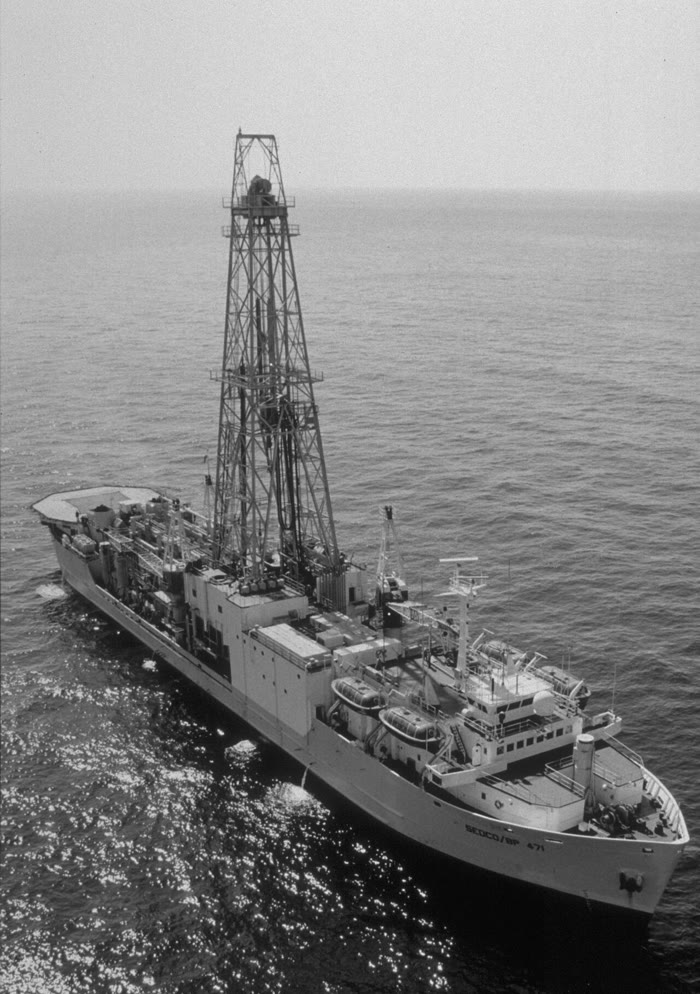
\includegraphics[width=0.36\linewidth]{images/book2/g11-odp-joides-resolution.jpg}

{\small O navio-sonda \emph{JOIDES Resolution}, que sucedeu o
\emph{Glomar Challenger}: a torre alta é a sua torre de perfuração, e o
navio leva mais de \qty{9000}{m} de tubos de perfuração. Fotografia: Ocean
Drilling Program, Texas A\&M University (domínio público).}
\end{omfigure}
% ledger: photo:g11-joides, usgs:glomar

Desde então, milhares de perfis magnéticos e centenas de furos de sondagem
foram reunidos num mapa da idade de todo o assoalho oceânico.

\begin{omfigure}
\begin{tikzpicture}
\begin{axis}[ommap, width=\linewidth, xtick=\empty, ytick=\empty, grid=none,
    axis background/.style={}, clip=true, name=map]
  \addplot graphics[xmin=-180, xmax=180, ymin=-90, ymax=90] {figdata/out/grade-11-seafloor_age.png};
  \addplot[black!60, line width=0.15pt] table {figdata/out/shared-geo-land.dat};
\end{axis}
\begin{axis}[at={(map.south)}, anchor=north, yshift=-0.35cm, scale only axis, width=0.55\linewidth, height=0.32cm,
    xmin=0, xmax=200, ymin=0, ymax=1, axis y line=none, axis x line*=bottom,
    xtick={0,20,...,180}, tick label style={font=\scriptsize},
    xlabel={idade do assoalho oceânico (milhões de anos); cinza: sem assoalho oceânico}, label style={font=\scriptsize},
    enlargelimits=false]
  \addplot graphics[xmin=0, xmax=200, ymin=0, ymax=1] {figdata/out/grade-11-seafloor_age-bar.png};
\end{axis}
\end{tikzpicture}

{\small A idade do assoalho oceânico. Mais jovem (vermelho) ao longo das
dorsais, ele fica mais velho à medida que se afasta delas, dos dois lados; o
assoalho mais antigo (azul e roxo) fica nas bordas dos oceanos, junto aos
continentes e ao longo das fossas. Dados: Seton e colaboradores (2020), em
células de 1 grau; contornos das terras: Natural Earth.}
\end{omfigure}
% ledger: data:b2-seafloor-age, data:ne-land (map computed in figdata/grade-11/seafloor_age.py)

O mapa confirma tudo de uma vez. Ao longo de cada dorsal, o assoalho é
jovem, e a sua idade cresce simetricamente à medida que se afasta dela.
Nenhum assoalho oceânico tem mais de cerca de \num{190} milhões de anos: o
mais antigo fica no oeste do Pacífico e ao largo da costa leste da América
do Norte (algumas pequenas bacias do leste do Mediterrâneo são contadas à
parte). A idade média do assoalho oceânico é de cerca de \num{64} milhões de
anos, e cerca de três quartos dele têm menos de 100 milhões de anos ---
enquanto os continentes guardam rochas muito mais antigas. O assoalho
oceânico é jovem porque está sempre sendo fabricado nas dorsais e, como Hess
percebeu, destruído em outro lugar: onde, é o assunto do
\cref{ch:g11:subduction-zones}.
% ledger: data:b2-seafloor-age (oldest_open_myr 192.5, share_younger_100 0.76 in figdata/grade-11/seafloor_age.py), seton:mean-age, usgs:hess

\section{Exercícios}

\begin{exercise}[$\star$]\label{exo:g11:drift-to-spreading:1}
Defina a \omterm{def:g11:drift-to-spreading:spreading}{expansão do assoalho oceânico}. Qual é a diferença entre a \omterm{def:g11:drift-to-spreading:spreading-rate}{taxa de
expansão total} e a \omterm{def:g11:drift-to-spreading:spreading-rate}{semitaxa de expansão} de uma dorsal?
\end{exercise}

\begin{exercise}[$\star$]\label{exo:g11:drift-to-spreading:2}
Por que uma lava só registra a direção do campo da Terra depois de esfriar
abaixo de cerca de \qty{580}{\celsius}? O que acontece com esse registro se
a rocha for mais tarde aquecida a \qty{700}{\celsius}?
\end{exercise}

\begin{exercise}[$\star$]\label{exo:g11:drift-to-spreading:3}
Um ecobatímetro ouve o eco do seu pulso \qty{5.2}{s} depois de enviá-lo.
Tomando a velocidade do som na água do mar como \qty{1500}{m/s}, a que
profundidade está o fundo do mar?
\end{exercise}

\begin{exercise}[$\star$]\label{exo:g11:drift-to-spreading:4}
Na escala de tempo de polaridade deste capítulo: há quanto tempo dura o
intervalo normal atual? Quanto durou o evento Jaramillo? Quantas inversões
ocorreram nos últimos cinco milhões de anos?
\end{exercise}

\begin{exercise}[$\star$]\label{exo:g11:drift-to-spreading:5}
As dorsais oceânicas têm cerca de \qty{65000}{km} de comprimento. A
circunferência da Terra é de cerca de \qty{40000}{km}. Quantas voltas à
Terra as dorsais dariam?
\end{exercise}

\begin{exercise}[$\star\star$]\label{exo:g11:drift-to-spreading:6}
Num perfil magnético, a fronteira entre os intervalos Brunhes e Matuyama
(\num{0.78} milhão de anos) fica a \qty{20}{km} do eixo da dorsal. Calcule a
semitaxa e a taxa total em centímetros por ano.
\end{exercise}

\begin{exercise}[$\star\star$]\label{exo:g11:drift-to-spreading:7}
Em outro perfil, a fronteira Gauss--Gilbert (\num{3.58} milhões de anos)
fica a \qty{45}{km} a oeste e a \qty{44}{km} a leste do eixo. Calcule a
semitaxa de cada lado e a taxa total. A expansão é simétrica?
\end{exercise}

\begin{exercise}[$\star\star$]\label{exo:g11:drift-to-spreading:8}
O local 19 da perfuração de 1968 fica a \qty{990}{km} do eixo da Dorsal
Mesoatlântica. Usando uma semitaxa de \qty{1.9}{cm} por ano, preveja a idade
do assoalho ali, e compare com os \num{49} milhões de anos do seu sedimento
mais antigo.
\end{exercise}

\begin{exercise}[$\star\star$]\label{exo:g11:drift-to-spreading:9}
Uma dorsal se expande com uma semitaxa de \qty{2}{cm} por ano. Usando a
escala de tempo deste capítulo, dê as distâncias ao eixo das fronteiras de
0.78, 0.99, 1.07, 1.77 e 1.95 milhão de anos, e desenhe as listras de um
lado, as normais em preto.
\end{exercise}

\begin{exercise}[$\star\star$]\label{exo:g11:drift-to-spreading:10}
A idade média do assoalho oceânico é de cerca de \num{64} milhões de anos; a
Terra tem cerca de \num{4.6} bilhões de anos. Que fração da idade da Terra é
isso? Que argumento de Hess isso apoia?
\end{exercise}

\begin{exercise}[$\star\star$]\label{exo:g11:drift-to-spreading:11}
Explique, com um desenho, por que o padrão das listras magnéticas de um lado
de uma dorsal é a imagem espelhada do padrão do outro lado. O que quebraria
essa simetria?
\end{exercise}

\begin{exercise}[$\star\star\star$]\label{exo:g11:drift-to-spreading:12}
Suponha que as dorsais, com \qty{65000}{km} de comprimento ao todo, se
expandam a uma taxa total média de \qty{5}{cm} por ano.
\begin{enumerate}
  \item Que área de novo assoalho oceânico elas fabricam a cada ano, em
        \unit{km^2}?
  \item O assoalho oceânico cobre cerca de \qty{2.9e8}{km^2}. Quanto tempo as
        dorsais levariam para fabricar tudo isso?
  \item Compare com o assoalho oceânico mais antigo, de cerca de \num{190}
        milhões de anos. O que deve acontecer com o assoalho oceânico tão
        depressa quanto ele é fabricado?
\end{enumerate}
\end{exercise}

\begin{exercise}[$\star\star\star$]\label{exo:g11:drift-to-spreading:13}
O evento Jaramillo durou de \num{0.99} a \num{1.07} milhão de anos atrás.
Qual é a largura da sua listra de cada lado de uma dorsal com semitaxa de
\qty{1.25}{cm} por ano, e de uma com \qty{7.5}{cm} por ano? A rocha
magnetizada fica a cerca de \qty{3}{km} abaixo da superfície do mar.
Explique por que o evento aparece claramente no perfil rápido deste
capítulo, mas quase nada no lento.
\end{exercise}

\begin{exercise}[$\star\star\star$]\label{exo:g11:drift-to-spreading:14}
Nos locais de 1968, o sedimento tem \qty{176}{m} de espessura no local 16,
cujo assoalho tem cerca de \num{11} milhões de anos, e apenas \qty{72}{m}
no local 20, com cerca de \num{67} milhões de anos. Calcule a taxa média com
que o sedimento se acumulou em cada local, em metros por milhão de anos. A
espessura do sedimento pode ser usada para datar o assoalho? O que se usa em
vez dela?
\end{exercise}

\begin{exercise}[$\star\star\star$]\label{exo:g11:drift-to-spreading:15}
Num perfil através de uma dorsal, a fronteira de \num{2.581} milhões de anos
fica a \qty{58}{km} a oeste e a \qty{70}{km} a leste do eixo.
\begin{enumerate}
  \item Calcule a semitaxa de cada lado e a taxa total.
  \item O assoalho a leste do eixo foi fabricado mais depressa que o
        assoalho a oeste. Depois de 10 milhões de anos a essas taxas, a que
        distância do eixo estaria o assoalho dessa idade de cada lado?
  \item Explique por que a distância entre as duas fronteiras dá a taxa
        total mesmo que a expansão não seja simétrica.
\end{enumerate}
\end{exercise}

\section{Problema: a idade do Atlântico Sul}

\begin{problem}[{Problema de fim de semana --- datar um oceano de três maneiras}]
\label{pb:g11:drift-to-spreading:1}
% ledger: dsdp3:table5, dsdp3:rate, data:b2-seafloor-age, earth:Rmean, ics:base.Cretaceous
% (values computed in figdata/grade-11/sediment_ages.py and seafloor_age.py)
Em 1968, o \emph{Glomar Challenger} perfurou sete furos através da Dorsal
Mesoatlântica perto da latitude \ang{30} Sul. A tabela dá, para cada local,
a sua distância ao eixo da dorsal, a idade do sedimento mais antigo sobre o
basalto (pelos seus fósseis) e, onde a listra abaixo dele foi identificada,
a idade dessa listra magnética, em milhões de anos.

\begin{center}
\small
\begin{tabular}{|c|c|c|c|}
\hline
local & distância ao eixo (\unit{km}) & idade do sedimento mais antigo & idade da listra magnética \\ \hline
16 & 191 & 11 & 9 \\ \hline
15 & 380 & 24 & 21 \\ \hline
18 & 506 & 26 & --- \\ \hline
17 & 643 & 33 & --- \\ \hline
14 & 727 & 40 & 38.5 \\ \hline
19 & 990 & 49 & 53 \\ \hline
20 & 1270 & 67 & 71 \\ \hline
\end{tabular}

{\small Dados: Deep Sea Drilling Project, Leg 3 (1970); as idades magnéticas
são o meio dos intervalos dados ali.}
\end{center}

\begin{center}
\begin{tikzpicture}
\begin{axis}[omrecord, width=0.82\linewidth, height=5.0cm, xmin=-50, xmax=16, ymin=0, ymax=140,
  xlabel={longitude ao longo de \ang{30} Sul (graus; negativa: oeste)}, ylabel={idade (milhões de anos)},
  tick label style={font=\small}, label style={font=\small}, clip=false]
\addplot[omDef, line width=0.8pt] table[x=lon, y=age] {figdata/out/grade-11-seafloor_age-profile.dat};
\draw[omRidge, densely dashed] (axis cs:-13.8,0) -- (axis cs:-13.8,140);
\node[font=\scriptsize, text=omRidge, anchor=south] at (axis cs:-13.8,140) {eixo da dorsal};
\fill (axis cs:-47.4,125.1) circle (1.5pt);
\node[font=\scriptsize, anchor=south west, inner sep=2pt] at (axis cs:-47.6,126) {América do Sul};
\node[font=\scriptsize, anchor=north west, align=left] at (axis cs:14.2,135) {África};
\fill (axis cs:13.8,129.8) circle (1.5pt);
\end{axis}
\end{tikzpicture}

{\small A idade do assoalho oceânico ao longo do paralelo \ang{30} Sul, da
América do Sul à África; a linha para onde o assoalho oceânico termina junto
a cada continente. Dados: Seton e colaboradores (2020).}
\end{center}

\medskip
\noindent\textbf{Parte I --- Os locais de perfuração.}
\begin{enumerate}
  \item Que local fica mais perto da dorsal, e qual mais longe? Como se
        comparam as suas idades?
  \item Por que a idade do sedimento mais antigo assentado sobre o basalto é
        próxima da idade do próprio basalto? Ela é um pouco mais velha ou um
        pouco mais jovem?
  \item Para cada local, calcule a razão entre a sua distância e a idade do
        seu sedimento mais antigo, em quilômetros por milhão de anos.
  \item Qual é a média dessas sete razões? Converta-a em centímetros por
        ano.
  \item Os locais 17 e 18 ficam a leste da dorsal, os outros a oeste dela. Os
        locais do leste seguem a mesma tendência que os do oeste? O que isso
        diz sobre a expansão?
\end{enumerate}

\medskip
\noindent\textbf{Parte II --- A taxa pelos sedimentos.}
\begin{enumerate}[resume]
  \item Se o assoalho se expandisse com uma semitaxa constante $u$, como a
        idade $t$ do assoalho dependeria da sua distância $d$ ao eixo?
  \item A reta pela origem que melhor se ajusta aos pontos tem a inclinação
        $u = \sum d\,t / \sum t^2$. Para os sete locais,
        $\sum d\,t = \num{208276}$ e $\sum t^2 = \num{10952}$ (em
        quilômetros e milhões de anos). Calcule $u$ em quilômetros por
        milhão de anos e em centímetros por ano.
  \item Qual é a \omterm{def:g11:drift-to-spreading:spreading-rate}{taxa de expansão total} do Atlântico Sul nessa latitude?
  \item Os cientistas da expedição escreveram que a taxa era ``um pouco
        menor que \qty{2}{cm} por ano''. Você concorda?
  \item Com essa taxa, preveja a idade do assoalho no local 20, e compare com
        o seu sedimento mais antigo.
\end{enumerate}

\medskip
\noindent\textbf{Parte III --- A taxa pelas listras magnéticas.}
\begin{enumerate}[resume]
  \item Só a partir do local 16 (\qty{191}{km}, listra de 9 milhões de
        anos), calcule uma semitaxa.
  \item Só a partir do local 20 (\qty{1270}{km}, listra de 71 milhões de
        anos), calcule uma semitaxa.
  \item Para os cinco locais com idade magnética, $\sum d\,t = \num{180329}$
        e $\sum t^2 = \num{9854}$. Calcule a melhor semitaxa.
  \item Em quantos por cento as taxas dadas pelos fósseis e pelas listras
        diferem? Os dois métodos concordam?
  \item Por que é importante que as duas idades tenham sido encontradas por
        métodos completamente diferentes?
\end{enumerate}

\medskip
\noindent\textbf{Parte IV --- Até a borda do oceano.}
\begin{enumerate}[resume]
  \item Ao longo de \ang{30} Sul, o eixo da dorsal fica na longitude
        \ang{13.8} Oeste e o assoalho oceânico termina junto à África em
        \ang{13.8} Leste. Quantos graus de longitude os separam?
  \item Numa esfera de raio \qty{6371}{km}, um grau de longitude mede
        $\qty{111.2}{km} \times \cos(\text{latitude})$. Calcule o
        comprimento de um grau a \ang{30} Sul, e a distância do eixo até a
        borda do assoalho oceânico junto à África.
  \item Se o assoalho tivesse sempre se expandido à taxa da Parte II, há
        quanto tempo o assoalho da borda teria se formado?
  \item O mapa das idades, que data o assoalho antigo pelas suas listras
        magnéticas, dá \num{130} milhões de anos na borda. Que semitaxa média
        isso implica? A abertura inicial do oceano foi um pouco mais rápida
        ou um pouco mais lenta que a abertura dos últimos 66 milhões de
        anos?
  \item Conclua: qual é a idade do assoalho oceânico mais antigo junto à
        África a \ang{30} Sul? O período Cretáceo começou há cerca de
        \num{143} milhões de anos: em que período o Atlântico Sul começou a
        se abrir ali?
\end{enumerate}
\end{problem}
